\chapter{$ISA^{2}$}

Hemos hablado anteriormente de qué son los sistemas \ac{ISA} a grandes rasgos y la principal novedad de $ISA^{2}$ frente a éstos, pero conviene entrar en detalle para explicar la metodología que hemos seguido y los problemas que nos hemos encontrado y solventado.

\section{Estructura de $ISA^{2}$}

Para poder explicar la metodología, antes debemos de preguntarnos cómo funciona todo el sistema de $ISA^{2}$, centrándonos en cada parte que lo compone para que resulte más fácil su comprensión. He aquí unas figuras ilustrativas que nos servirán como punto de referencia durante todo el capítulo:


\begin{figure}[h]
  \centering
  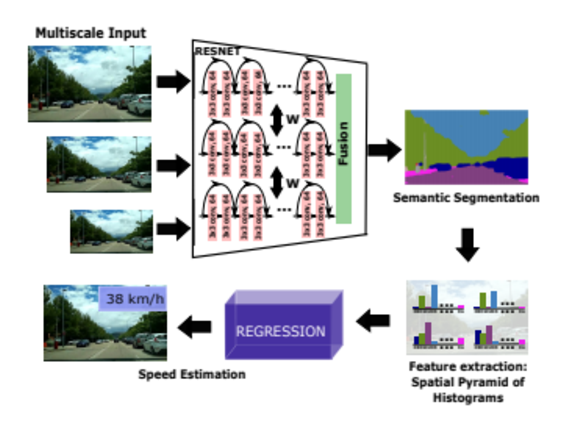
\includegraphics[width=8cm]{Figuras/Figura_Esquema_ISA2_Version_1_SegSem.eps}
  \caption{Esquema $ISA^{2}$ Antiguo}
  \label{fig:Isa_v1}
\end{figure}


Como se puede ver al pie de la figura \ref{fig:Isa_v1}, este fue el esquema utilizado para la primera versión de $ISA^{2}$ \cite{isa2} y funcionaba de la siguiente manera:


\begin{itemize}
\item En primera instancia el sistema recogía un set de imágenes que se correspondía con situaciones de tráfico tanto en autovía (o autopista) como en núcleos urbanos. Cuando el sistema tenía que procesar una imagen, ésta venía en diferentes escalas puesto que el modelo de ``DeepLab'' de \ac{SS} trabajaba así. Este modelo tenía como base una \ac{CNN}, es decir, una Red Neuronal Convolucional \cite{cnn}.
 
\item Este tipo de tecnología es la que posibilitó entonces, y ahora, la \ac{SS} de las imágenes.

\subsection{Segmentación Semántica}

Pero, ¿qué es la \ac{SS}? ¿Y por qué es tan útil en este proyecto?


En el capítulo anterior hablamos de una forma resumida en qué consiste la \ac{SS} y su uso en el proyecto, pero es tan solo la punta del iceberg.


La \ac{SS} es un proceso por el cual los píxeles de una imagen son dotados de distintos valores para poder diferenciarlos en etiquetas unos de otros y así reconocer los elementos que componen dicha imagen. 


Por ejemplo: Una fotografía de una persona, un coche y un perro. A priori, todos los píxeles de la imagen no están categorizados y no se sabe qué partes de la imagen corresponden a la persona, al coche, y al perro. Gracias a la segmentación semántica los píxeles de la imagen adquieren los valores de las etiquetas referentes a ``persona'', a ``coche'' y a ``perro''; y son fácilmente diferenciables.

Cuando hablamos de ``diferenciables'' nos referimos a los programas y soluciones que trabajan con este tipo de tecnologías. Más adelante usaremos unos códigos en MatLab que trabajan con estas etiquetas, pero es conveniente saber el porqué de esa ``diferenciabilidad'' a la que se hace alusión.

\item Tras este proceso, mediante unos códigos de Matlab se recogían los datos de los píxeles ya segmentados y se organizaban en histogramas. Basándonos en los histogramas generados, usábamos una estrategia llamada \ac{SPP} \cite{spp} para crear un descriptor de imagen.

\item Por último, el descriptor generado en el paso anterior se pasaba a diferentes sistemas de regresión. Para cada uno de ellos se añadía \ac{SI} \cite{spp} usando \ac{SPP} de hasta 3 niveles para poder compararlos entre sí y saber cuál era mejor. Para ello cogíamos los mejores resultados de cada uno de todos los niveles usados en los mismos.

\end{itemize}


Fue de esta manera como se pudo ejecutar con eficacia este sistema \cite{isa2}. Sin embargo, con el paso de los años surgieron nuevos modelos de \ac{SS} más eficaces y precisos, y fruto de ello es el sistema que hemos utilizado en esta nueva versión: Swiftnet \cite{swiftnet}.


\begin{figure}[H]
  \centering
  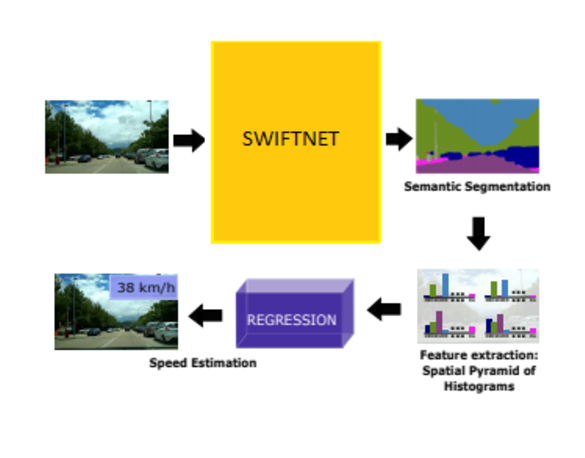
\includegraphics[width=8cm]{Figuras/Figura_Esquema_ISA2_Version_2.eps}
  \caption{Esquema $ISA^{2}$ Actual}
    \label{fig:Isa_v2}
\end{figure}


Como se puede comprobar, el esquema de la figura \ref{fig:Isa_v2} sigue el mismo camino que el de la primera versión, salvo por unas modificaciones al principio que pasamos a explicar a continuación:

\begin{enumerate}

\item Las imágenes de entrada al modelo de \ac{SS} no llegan en diferentes escalas como se podría intuir. La razón de por qué es así es ``Swiftnet'': El modelo admite tanto imágenes en diferente escala como imágenes en una única.


Sin embargo, para este proyecto hemos optado por la recomendación de los autores \cite{github_swiftnet} y hemos decidido hacerlo con una única escala. De esta manera hemos obtenido los resultados esperados con la dataset de Cityscapes \cite{cityscapes} que ellos mismos utilizaron \cite{swiftnet}.

\item La segunda, y última, modificación es la más obvia: la sustitución del modelo de ``DeepLab'' \cite{deeplab} por el modelo de ``Swiftnet'' \cite{swiftnet}.

A diferencia del primero, ``Swiftnet'' es un modelo que opera en tiempo real (``Real-Time'') de tal modo que cuando procesa una imagen lo hace en el momento, mientras que ``DeepLab'' tiene que esperar a que se recoja un set de imágenes para luego ir procesándolas.

\end{enumerate}


En el siguiente capítulo hablaremos acerca de la implementación de ``Swiftnet'' y de cómo es mejor para los campos de aplicación, especificados anteriormente, con respecto a ``DeepLab''.